\documentclass{article}

\usepackage{style}


\usepackage{Sweave}
\begin{document}

\Sconcordance{concordance:campbell_protocol.tex:campbell_protocol.Rnw:%
1 5 1 1 0 137 1 1 6 8 0 1 2 2 1 1 4 6 0 1 2 82 1}


\vspace{20mm}


\begin{Huge}
\begin{center}
\textbf{Systematic Review Protocol: The direct effect of malaria control on productivity: a systematic review}
\end{center}
\end{Huge}



\vspace{5mm}

\begin{changemargin}{2.5cm}{2.5cm} 
\begin{center}
\begin{large}
Joe Brew \hfill \emph{joe.brew@isglobal.org} \\
Laia Cirera Crivillé \hfill \emph{laia.cirera@isglobal.org} \\ 
Elisa Sicuri \hfill \emph{elisa.sicuri@isglobal.org} \\ 
\end{large}
\end{center}
\end{changemargin}


\vspace{6mm}

\begin{center}
\begin{large}
Institut de Salut Global de Barcelona 
\end{large}
\end{center}


\begin{changemargin}{3cm}{3cm} 

\begin{center}
\textbf{Summary}
\end{center}

\emph{The literature regarding the economic effect of malaria control and prevention interventions on those targeted is scant, varies in terms of units and metrics, and stems from a diversity of times and locales. These factors make the comparison of different interventions difficult. By carrying out a systematic review of the available literature pertaining to the direct economic impact of malaria control and prevention activities, we will aggregate information to generate standardized measurements of interventions' effects, informing both the scientific discussion on malaria as well as public health practice.}

\end{changemargin}

\vfill  


\section*{Background}

\subsection*{The issue}


The economic effect of infection with malaria is poorly understood, but establishing the cost-effectiveness of malaria control interventions is crucial, particularly in light of the fact that malaria disproportionately impacts low-income countries. Though macro-level analyses suggest that a reduction in malaria's burden could be causally associated with increased economic growth \cite{Sachs2002}, the direct impact on worker productivity, income, and expenditure is unclear. \\


\noindent Public health authorities are interested in quantifying the overall effect of malaria control on worker health, as measured in DALY's, QALY's, and other metrics of morbidity and mortality. But quantifying the short-term and direct impact of malaria infection (or, inversely, prevention) on a worker's productivity is a more useful and actionable metric for those who finance malaria control activities outside of the public sector, especially private firms. Much of the available literature on the topic of malaria's economic burden is either exclusively macroeconomic (overly general) \cite{Bloom2004} or narrowly understands costs to be only the value of work-time lost, as translated to worker wages (overly specific)\cite{Chima2003}. A critical and systematic review of available evidence on the totality of direct costs related to malaria and its control is sorely needed, and would serve not only to further the scientific discussion regarding the economics of malaria, but could inform the advisability and sustainability of interventions carried out by both the private and public sectors. 

\subsection*{The interventions}

Malaria control is constituted by many interventions: the distribution of insecticide-treated bed nets (ITNs), indoor residual spraying (IRS) of buildings, mass drug administration (MDA), larval control (LC), biological control (BC), area spraying (AS), pre-exposure prophylasis (PEP) and, more recently, the malaria vaccine (MV). These interventions have been evaluated in multiple instances and areas both in terms of their implementation costs, as well as their benefits in human health and disease prevention. However, analyses focusing on the \emph{economic} benefits are scattered, use different currencies and times, do not follow a standardized approach to defining "productivity", and do not reach consensus in regards to the prospective time-frame for which the effect of a disease (or its prevention) should be counted.\\  

\subsection*{How we assess interventions}

A clear comparison between different interventions in regard to their effects on the economic well-being of those targeted necessitates both (a) a clear understanding and delineation of what those effects are (both in terms of kind and time), and (b) a standardization of the pricing units used to measure those effects. \\ 

\noindent In regards to the delineation of what constitutes an effect, we follow the below flow chart.

\begin{center}
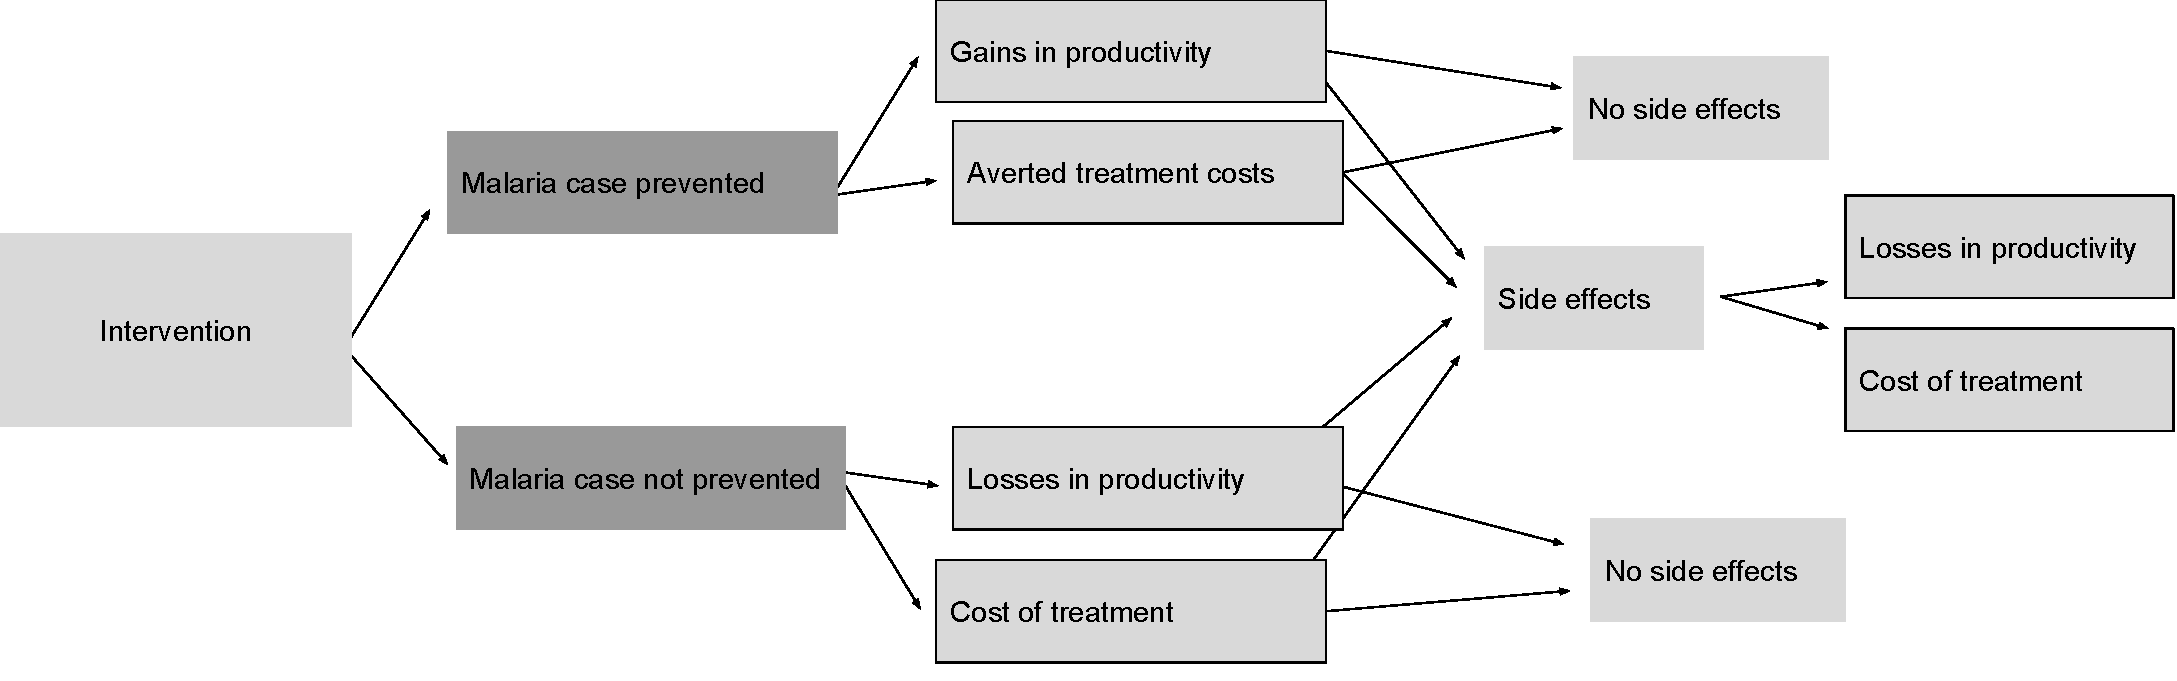
\includegraphics[width=1\textwidth]{logic_flow.pdf}
\end{center}

\noindent In the flow chart, the calculation of prevalence/incidence occurs at the dark grey boxes, whereas the costing of economic effects occurs at boxes with black borders. In all cases, we limit the effect timeframe to exactly one year following the intervention, and adjust for age, pregnancy status, and overal population malaria prevalence whenever possible. For all costs, we use 2015 United States dollars. Costs are standardized to a per-person basis, and converted to direct return on investment. \\

\noindent This standardized approach allows us to compare the economic effect of malaria control and prevention interventions across time and space.


\subsection*{Why it is important to do the review}

A systematic review of the literature on the direct economic impact of malaria control and prevention is sorely needed. Particularly in light of the current push for eradication, standardized comparisons of interventions is important to researchers, policy-makers, and public health practitioners. \\

\noindent Much of the current literature on the economic impact of malaria control and prevention focuses on indirect costs and benefits \cite{Gallup1998}, is only quasi-scientific \cite{rbm2011}, is exclusively macroeconomic \cite{Hsiao2015} \cite{Zafar2007} \cite{Carstensen2006}, and overwhelmingly restricted to outcomes in health alone. Studies which estimate the direct economic effect of those targeted by interventions are both difficult to find and vary in regards to quality, interventions assessed,  outcomes measured, time, geography, and units used. A systematic review is needed not only to identify which studies are of utility for those seeking to answer questions regarding the economic effect of malaria control, but also to standardize measurements and make comparisons in a way that is useful and actionable. \\

\noindent We anticipate that the results of this review will have notable application on the science, policy, and practice of malaria control and prevention. In particular, we believe that the direct comparisons and quantification of return on investment made possible by our review will be of great interest to business investors seeking to reduce absenteeism and increase productivity of workers in malaria-endemic regions as well as governments and health institutions in low-income countries which are keen on economic development. 



\section*{Objectives}

This review has one \textbf{primary} objective: \\ 

\begin{itemize}
\item Standardize, quantify and compare the direct economic impact of malaria control and prevention interventions on those targetted. \\
\end{itemize}


\noindent \textbf{Secondary} objectives include: 
\begin{itemize}
  \setlength\itemsep{-0.2em}


\item Provide an explanation for differing results over time and space 
\item Translate all findings into "return on investment", so as to be of more interest to those in the private sector
\item Create and document a framework for the replication of this review over time and for other diseases  
\item Augment the review through the inclusion of the estimation of side-effects and direct treatment costs taking from the general economic and biomedical literature
\end{itemize}


\section*{Methodology}

\subsection*{Criteria for including studies in the review}

\noindent \textbf{Inclusion criteria} \\


\begin{itemize}
\item \emph{Study design}
\item \emph{Timeframe}
\item \emph{Geography}
\item \emph{Control/comparison}
\item \emph{Measures}
\item \emph{Duration of follow-up}
\item \emph{Types of interventions}
\item \emph{Types of participants}
\item \emph{Measures}
\item \emph{Types of outcome measures}
\end{itemize}


\noindent \textbf{Exclusion criteria} \\


\subsection*{Search Strategy}

\noindent \textbf{} \\
\noindent \textbf{} \\


\subsection*{Description of methods used in primary research}


\subsection*{Criteria for determination of independent findings}


\subsection*{Details of study coding categories (including methodological quality or risk of bias coding)}

\subsection*{Statistical procedures and conventions}

\subsection*{Treatment of qualitative research}



\section*{Table example}

\section*{Sources of Support}

Describe the source(s) of support for the proposed review. 

\section*{Declarations of interest}

Please declare any potential conflicts of interest.

\section*{Review authors}

\subsection*{Lead review author}

Name: Joe Brew\\
Title: Pre-doctoral fellow\\
Affiliation: Institut de Salut Global de Barcelona\\
Address: c/ Rosselló, 132\\
City, State, Province or County: Barcelona\\
Postal Code: 08036\\
Country: Spain\\
Phone: +34 666 66 80 86\\
Email: joe.brew@isglobal.org\\
Role: Retrieval and statistical expertise\\


\subsection*{Co-authors}

Name: Laia Cirera Crivillé\\
Title: Researcher\\
Affiliation: Institut de Salut Global de Barcelona\\
Address: c/ Rosselló, 132\\
City, State, Province or County: Barcelona\\
Postal Code: 08036\\
Country: Spain\\
Email: laia.cierera@isglobal.org\\
Role: Content expertise\\


\vspace{5mm}

\noindent Name: Elisa Sicuri\\
Title: Professor of Economics\\
Affiliation: Institut de Salut Global de Barcelona\\
Address: c/ Rosselló, 132\\
City, State, Province or County: Barcelona\\
Postal Code: 08036\\
Country: Spain\\
Email: elisa.sicuri@isglobal.org\\
Role: Methodological expertise\\


\section*{Preliminary timeframe}

\begin{itemize}
  \setlength\itemsep{-0.2em}
\item April-May 2016: protocol redaction and approval
\item May-June 2016: systematic retrieval and designation of articles for review
\item July-August 2016: review of articles
\item September-October 2016: analysis and synthesis, preparation of manuscript for publication
\item November 2016: Submission for publication
\end{itemize}

\section*{Plans for updating the review} 

The review will be updated, using identical methods, every two years, beginning in November 2018 (two years after initial submission for publication). Joe Brew will be responsible for coordinating updates.

\section*{Authors’ Responsibilities}
By completing this form, you accept responsibility for preparing, maintaining and updating the review in accordance with Campbell Collaboration policy. The Campbell Collaboration will provide as much support as possible to assist with the preparation of the review. \\

\noindent A draft review must be submitted to the relevant Coordinating Group within two years of protocol publication. If drafts are not submitted before the agreed deadlines, or if we are unable to contact you for an extended period, the relevant Coordinating Group has the right to de-register the title or transfer the title to alternative authors. The Coordinating Group also has the right to de-register or transfer the title if it does not meet the standards of the Coordinating Group and/or the Campbell Collaboration. \\

\noindent You accept responsibility for maintaining the review in light of new evidence, comments and criticisms, and other developments, and updating the review at least once every five years, or, if requested, transferring responsibility for maintaining the review to others as agreed with the Coordinating Group.

\section*{Publication in the Campbell Library}

The support of the Campbell Collaboration and the relevant Coordinating Group in preparing your review is conditional upon your agreement to publish the protocol, finished review and subsequent updates in the Campbell Library. Concurrent publication in other journals is encouraged. However, a Campbell systematic review should be published either before, or at the same time as, its publication in other journals. Authors should not publish Campbell reviews in journals before they are ready for publication in the Campbell Library. Authors should remember to include a statement mentioning the published Campbell review in any non-Campbell publications of the review. \\


\noindent I understand the commitment required to undertake a Campbell review, and agree to publish in the Campbell Library. Signed on behalf of the authors: \\

\vspace{10mm}
\noindent Form completed by:\\
\noindent Date: 


\bibliography{library}{}
\bibliographystyle{apalike}  




\end{document}
